\section{Posicionamiento}

Se refiere a la posibilidad de posicionar un elemento HTML en la página del sitio web. La propiedad para posicionar un elemento es \textbf{position}, la cual tiene algunos valores importantes a conocer:
\begin{itemize}
    \item \textbf{static}: se mantiene fijo según el flujo de elementos de la página, aún después de deslizarse hacía bajo en el sitio. Es es valor por defecto y no se puede posicionar fuera del flujo de elementos.
    \item \textbf{fixed}: se posiciona en una parte en específico de la página, aún después de deslizarse hacía abajo en el sitio, por lo que no sigue el flujo de elementos, esto puede provocar \textbf{superposición de elementos}.
    \item \textbf{relative}: se posiciona en una parte en específico de la página, pero se mantiene fija en dicha posición después de deslizar hacía abajo en el sitio (puede causar superposición de elementos).
    \item \textbf{absolute}: se posiciona en una parte en específico de la página, tomando como referencia la posición de su etiqueta padre más próxima, si no tiene, tomara esta referencia del documento en sí (body); se mantiene fija en dicha posición después de deslizar hacía abajo en el sitio (puede causar superposición de elementos).
\end{itemize}

Para posicionar un elemento en alguna parte en específico de la página, requerimos de las propiedad \textit{top}, \textit{left}, \textit{bottom}, \textit{right} y las \textit{unidades de valores}. Dejaremos un ejemplo sobre los posicionamientos de etiquetas y su resultado en la \textit{Figura \ref{fig: 25}}:
\begin{lstlisting}
estilos.css
    /* Se mantiene fijo en el flujo del documento. */
    .static p {
        position: static;
        /* Se ignoran las propiedades "top" y "left" debido a la posición estática. */
        top: 200px;
        left: 150px;
        width: 100px;
        height: 100px;
        background-color: red;
    }
    /* Se posiciona donde se desee, fuera del flujo del documento. */
    .fixed p {
        position: fixed;
        /* A 150px y 150px de la esquina superior izquierda. */
        top: 150px;
        left: 150px;
        width: 100px;
        height: 100px;
        background-color: blue;
        color: white;
    }
    /* Se posiciona donde se desee, dentro del flujo del documento. */
    .relative {
        position: relative;
        /* A 100px y 50px de la esquina superior izquierda. */
        top: 100px;
        left: 50px;
        width: 100px;
        height: 100px;
        background-color: coral;
    }
    /*
        Se posiciona donde se desee y con respecto a su etiqueta padre,
        en este caso, "body", fuera del flujo del documento.
    */
    .absolute {
        position: absolute;
        /* A 100px de la esquina superior izquierda. */
        top: 100px;
        width: 100px;
        height: 100px;
        background-color: darkgreen;
    }
    body {
        height: 5000px;
    }

prueba.html
    <div class="static">
        <p>Este párrafo tiene static position.</p>
    </div>
    <div class="fixed">
        <p>Este párrafo tiene fixed position.</p>
    </div>
    <div class="relative">
        <p>Este párrafo tiene relative position.</p>
    </div>
    <div class="absolute">
        <p>Este párrafo tiene absolute position.</p>
    </div>
\end{lstlisting}
\begin{figure}[H]
    \centering
    \caption{Diferencia entre valores de propiedad \textit{position}}
    \label{fig: 25}
    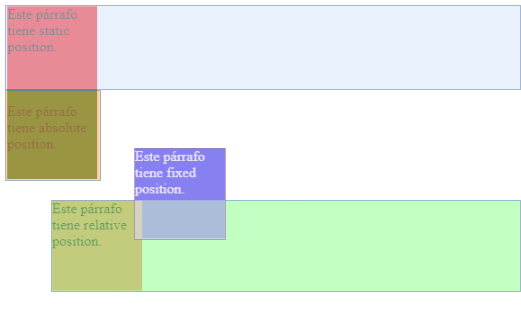
\includegraphics[width=14cm]{ss/position.png}
\end{figure}

Debe ejecutar este código en su buscador, ya que las diferencias visuales solamente se pueden apreciar cuando se desplaza sobre la página web.



\section{Floating}

La propiedad \textbf{float} de CSS permite que los elementos alrededor de otro "floten" o lo rodeen (usualmente utilizado en imágenes). Los valores que se aceptan son:
\begin{itemize}
    \item \textbf{left}: los elementos flotan a la izquierda.
    \item \textbf{right}: los elementos flotan a la derecha.
    \item \textbf{none}: los elementos no flotan (valor predeterminado).
    \item \textbf{inline-start}: los elementos flotan al principio de un contenedor o elemento padre.
    \item \textbf{inline-end}: los elementos flotan al final de un contenedor o elemento padre.
    \item \textbf{ihnerit}, \textbf{initial} y \textbf{unset}.
\end{itemize}

Los elementos que tiene la propiedad \textit{float} se posicionan en el extremo izquierdo o derecho (dependiendo si se estableció el valor \textit{left} o \textit{right} respectivamente) del contenedor donde están almacenados (body, div, section, etc.), y el resto de elementos los rodean. Dejaremos un ejemplo sobre los elementos flotantes y su resultado en la \textit{Figura \ref{fig: 26}}:
\begin{lstlisting}
estilos.css
    /* Muestra los elementos contenidos como bloques. */
    .block {
        display: block;
        height: 200px;
    }
    /* Los elementos flotan a la izquierda. */
    .left {
        float: left;
    }
    /* Los elementos flotan a la derecha. */
    .right {
        float: right;
    }

prueba.html
    <div class="block">
        <div class="left">
            <img src="https://www.zooplus.es/magazine/wp-content/uploads/2022/05/Cuanto-pesa-un-gato-2.jpeg"
            alt="https://images.unsplash.com/photo-1591871937631-2f64059d234f?ixlib=rb-4.0.3&ixid=MnwxMjA3fDB8MHxleHBsb3JlLWZlZWR8MXx8fGVufDB8fHx8&w=1000&q=80"
             width="200px" />
        </div>
        <p>Este párrafo flota al lado derecho de la imagen.</p>
    </div>
    <div class="block">
        <div class="right">
            <img src="https://www.zooplus.es/magazine/wp-content/uploads/2022/05/Cuanto-pesa-un-gato-2.jpeg"
            alt="https://images.unsplash.com/photo-1591871937631-2f64059d234f?ixlib=rb-4.0.3&ixid=MnwxMjA3fDB8MHxleHBsb3JlLWZlZWR8MXx8fGVufDB8fHx8&w=1000&q=80"
            width="200px" />
        </div>
        <p>Este párrafo flota al lado izquierdo de la imagen.</p>
    </div>
\end{lstlisting}
\begin{figure}[H]
    \centering
    \caption{Diferencia entre valores de propiedad \textit{float}}
    \label{fig: 26}
    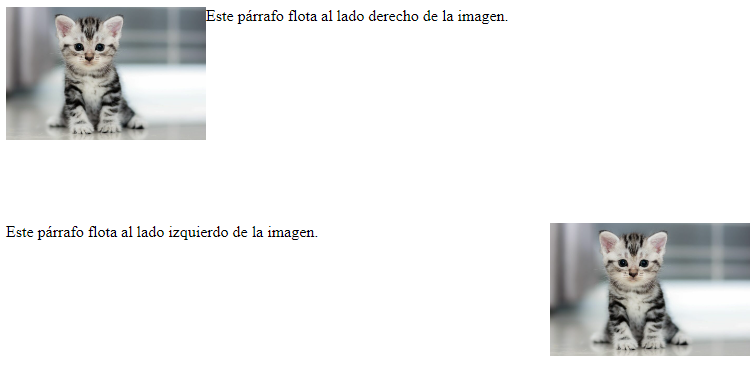
\includegraphics[width=14cm]{ss/float.png}
\end{figure}

En caso de que existan múltiples elementos con la propiedad \textit{float} uno al lado del otro, estos se posicionarán sin más uno enseguida del otro.



\section{Propiedades para la visualización de elementos}

Recordemos que todo elemento HTML es una caja, con su margen, \textit{padding}, borde y contenido; el buscador visualizará estos estos elementos de dos maneras principales:
\begin{itemize}
    \item \textbf{block-element}: elementos bloques, el buscador pondrá los elementos uno encima de otro (apilados), abarcando el 100\% del ancho de la página, a pesar de que el contenido de la etiqueta no lo abarque. Por lo general, muchas etiquetas tienen este tipo de visualización por defecto.
    \item \textbf{inline-elements}: elementos en línea, el buscador pondrá los elementos uno al lado del otro, ocupando solamente el ancho que requiera su contenido. Por lo general, las etiquetas \textbf{a} tienen este tipo de visualización por defecto.
\end{itemize}

Los dos conceptos anteriores servirán para explicar el ejemplo y figura del tema anterior, así como posteriores. La \textit{Figura \ref{fig: 27}} muestra la apariencia de ambas visualizaciones:
\begin{figure}[H]
    \centering
    \caption{Aspecto de las visualizaciones \textit{block} e \textit{inline}}
    \label{fig: 27}
    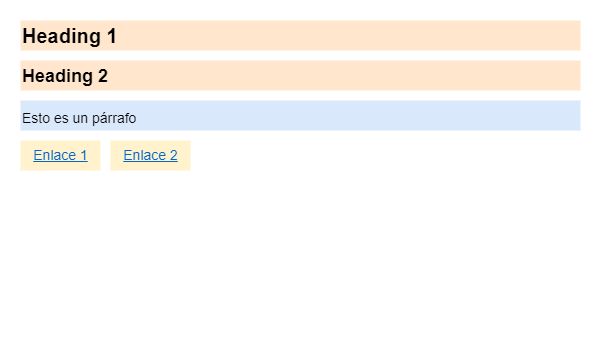
\includegraphics[width=12cm]{ss/display.png}
\end{figure}

Veremos entonces a continuación como modificar esta visualización con CSS.


\subsection{display}

La propiedad \textbf{display} de CSS acepta los siguientes valores:
\begin{itemize}
    \item \textbf{block}: visualiza los elementos HTML como elementos bloque, pudiendo cambiar su ancho y alto.
    \item \textbf{inline}: visualiza los elementos HTML como elementos en línea, no pudiendo cambiar su ancho y alto.
    \item \textbf{none}: no visualiza el elemento HTML, lo esconde, como si no estuviera presente, mostrando únicamente el contenedor que lo almacena.
    \item \textbf{inline-block}: visualiza los elementos HTML como elementos en línea, pero teniendo la posibilidad de asignar un ancho o alto al elemento.
\end{itemize}

Dejaremos un ejemplo sobre los posicionamientos de etiquetas y su resultado en la \textit{Figura \ref{fig: 28}}, inspeccionando cada elemento para que se note la diferencia entre todas:
\begin{lstlisting}
estilos.css
    /* Visualiza el elemento como bloque. */
    .block {
        display: block;
    }
    .block p {
        /* Hereda la visualización del bloque de su padre. */
        display: inherit;
        /* Establece tamaño al elemento. */
        width: 100px;
        height: 100px;
        background-color: red;
    }
    /* Visualiza el elemento como en línea. */
    .inline {
        display: inline;
    }
    .inline p {
        display: inherit;
        width: 100px;
        height: 100px;
        background-color: blue;
        color: white;
    }
    /* Visualiza el elemento como descartado. */
    .none {
        display: none;
    }
    /* Visualiza el elemento como bloque en línea. */
    .inline-block {
        display: inline-block;
    }
    .inline-block p {
        display: inherit;
        width: 100px;
        height: 100px;
        background-color: aqua;
    }

prueba.html
    <div class="block">
        <p>Este párrafo tiene block display.</p>
        <p>Este párrafo tiene block display.</p>
    </div>
    <div class="inline">
        <p>Este párrafo tiene inline display.</p>
        <p>Este párrafo tiene inline display.</p>
    </div>
    <div class="none">
        <p>Este párrafo no se incluirá en la visualización.</p>
    </div>
    <div class="inline-block">
        <p>Este párrafo tiene inline-block display.</p>
    </div>
\end{lstlisting}
\begin{figure}[H]
    \centering
    \caption{Diferencia entre valores de propiedad \textit{display}}
    \label{fig: 28}
    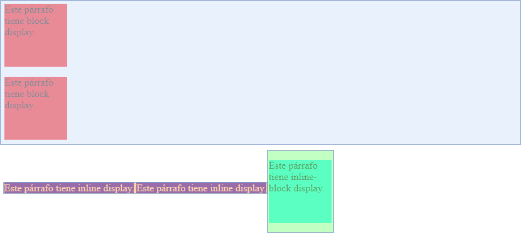
\includegraphics[width=14cm]{ss/prop-display.png}
\end{figure}

Vea que, a pesar de haber definido un tamaño para los elementos \textit{inline}(width=100px y height=100px), estos no sufren dichos cambios a su tipo de display, si tuvieran el valor \textit{block} o \textit{inline-block}, podríamos alterar su tamaño. Por otro lado, el elemento con display \textit{none} no aparece en el resultado del ejemplo, debido a que este no posee un espacio por abarcar en la visualización de la página, existe en el DOM, pero no abarca espacio visualmente.


\subsection{visibility}

La propiedad \textbf{visibility} de CSS esconde un elemento HTML, pero mantiene su espacio requerido, a diferencia de \textit{display: none}, que esconde el elemento y omite su espacio requerido. Los valores aceptados de esta propiedad son:
\begin{itemize}
    \item \textbf{hidden}: esconde el elemento.
    \item \textbf{visible}: muestra el elemento.
    \item \textbf{collapse}: para elementos regulares, este valor se comporta como \textit{hidden}; para las columnas y grupo de columnas y filas, este valor esconde la celda y el espacio que debería tener (como \textit{display: none}); para elementos \textit{collapsed flex}, este valor esconde los elementos y el espacio que deberían tener.
    \item \textbf{inherit}, \textbf{initial} y \textbf{unset}.
\end{itemize}

Dejamos un ejemplo y su resultado en la \textit{Figura \ref{fig: 29}}:
\begin{lstlisting}
estilos.css
    /* Esconde la visibilidad del elemento. */
    .hidden {
        visibility: hidden;
    }
    /* Muestra la visibilidad del elemento. */
    .visible {
        visibility: visible;
    }

prueba.html
    <div class="hidden">
        <h1>Este heading no se ve.</h1>
    </div>
    <div class="visible">
        <h1>Este heading si se ve.</h1>
    </div>
\end{lstlisting}
\begin{figure}[H]
    \centering
    \caption{Diferencia entre valores de propiedad \textit{visibility}}
    \label{fig: 29}
    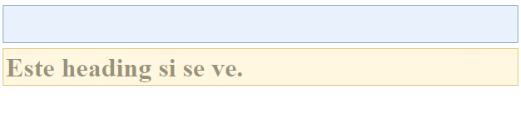
\includegraphics[width=10cm]{ss/visibility.png}
\end{figure}

Como podemos ver, esta propiedad esconde el elemento, pero mantiene su espacio en la página, a diferencia de la propiedad \textit{display none}.


\subsection{clear}

La propiedad \textbf{clear} de CSS ayuda a evitar que los elementos seguidos a uno que tiene la propiedad \textit{float} activa floten, es decir, \textbf{clear} evita que un elemento flote alrededor de otro. Los valores aceptados son:
\begin{itemize}
    \item \textbf{right}: evita flotar a la derecha de elementos con float.
    \item \textbf{left}: evita flotar a la izquierda de elementos con float.
    \item \textbf{both}: evita flotar en ambos lados de elementos con float.
    \item \textbf{none}: no evita flotar alrededor de elementos (valor predeterminado).
    \item \textbf{ihnerit}, \textbf{initial} y \textbf{unset}.
\end{itemize}

Dejamos un ejemplo y su resultado en la \textit{Figura \ref{fig: 30}}:
\begin{lstlisting}
estilos.css
    /* Los elementos flotan a la derecha de un elemento. */
    .floating {
        float: right;
    }
    /* Los elementos evitan flotar en ambos sentidos de un elemento. */
    .clearing {    
        clear: both;
    }
    /* Agrega borde sólido de 1 píxel a la imagen. */
    img {
        border-style: solid;
        border-width: 1px;
    }

prueba.html
    This paragraph is above the div element 
    and is not affected by the float right property. 
    <br/><br/>
    <div class="floating">
        <img src="http://www.sololearn.com/uploads/css_logo.png" height="300px"/>
    </div>
    This paragraph comes after the div element 
    and is affected by the float right property. 
    <div class="clearing">
        This paragraph is out of the floating group 
        and is not affected by the float right property.
    </div>
\end{lstlisting}
\begin{figure}[H]
    \centering
    \caption{Diferencia entre valores de propiedad \textit{clear}}
    \label{fig: 30}
    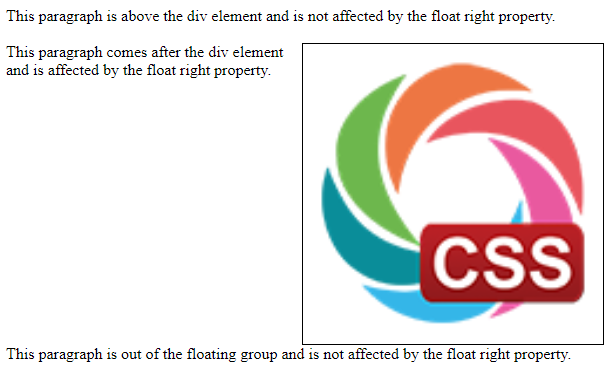
\includegraphics[width=12cm]{ss/clear.png}
\end{figure}


\subsection{overflow}

Recordemos que cada elemento HTML está contenido en una caja, cuando no establecemos el alto de la caja, este se ve ajustado automáticamente al contenido de la caja, sin embargo, si establecemos un alto y el contenido sobrepasa esta medida, se dice que ocurre un \textbf{desbordamiento} (\textit{overflow}), entonces, CSS tiene la propiedad \textbf{overflow}, que permite manejar el comportamiento del desbordamiento de contenido de los elementos. Los valores que acepta son:
\begin{itemize}
    \item \textbf{visible}: muestra completo el contenido desbordado del elemento (valor predeterminado).
    \item \textbf{scroll}: el contenido que sobresale es recortado y añade una barra de desplazamiento vertical y horizontal al elemento para ver el contenido que se desborda.
    \item \textbf{hidden}: el contenido que sobresale es recortado y no puede ser visto.
    \item \textbf{auto}: si el contenido es recortado, se añade una barra de desplazamiento vertical al elemento para ver el contenido que se desborda.
    \item \textbf{inherit}, \textbf{initial} y \textbf{unset}.
\end{itemize}

Dejamos un ejemplo y su resultado en la \textit{Figura \ref{fig: 31}}:
\begin{lstlisting}
estilos.css
    /* Pone los elementos uno al lado del otro. */
    .inline-block {
        display: inline-block;
    }
    /* Agrega un marge izquierdo de 10 píxeles. */
    p {
        margin-left: 10px;
    }
    /*
        Clases que reciben la propiedad "display" de su padre, se agrega un
        tamaño, borde y color para visualizar mejor el elemento, y se establece
        la propiedad "overflow".
    */
    .visible {
        display: inherit;
        width: 100px;
        height: 100px;
        border-style: solid;
        border-width: 1px;
        background-color: red;
        overflow: visible;
    }
    .hidden {
        display: inherit;
        width: 100px;
        height: 100px;
        border-style: solid;
        border-width: 1px;
        background-color: red;
        overflow: hidden;
    }
    .scroll {
        display: inherit;
        width: 100px;
        height: 100px;
        border-style: solid;
        border-width: 1px;
        background-color: red;
        overflow: scroll;
    }
    .auto {
        display: inherit;
        width: 100px;
        height: 100px;
        border-style: solid;
        border-width: 1px;
        background-color: red;
        overflow: auto;
    }

prueba.html
    <div class="inline-block">
        <p class="visible">Lorem ipsum dolor sit amet, consectetur adipiscing elit, sed do eiusmod tempor incididunt ut labore et dolore magna aliqua.</p>
        <p class="hidden">Lorem ipsum dolor sit amet, consectetur adipiscing elit, sed do eiusmod tempor incididunt ut labore et dolore magna aliqua.</p>
        <p class="scroll">Lorem ipsum dolor sit amet, consectetur adipiscing elit, sed do eiusmod tempor incididunt ut labore et dolore magna aliqua.</p>
        <p class="auto">Lorem ipsum dolor sit amet, consectetur adipiscing elit, sed do eiusmod tempor incididunt ut labore et dolore magna aliqua.</p>
    </div>
\end{lstlisting}
\begin{figure}[H]
    \centering
    \caption{Diferencia entre valores de propiedad \textit{overflow}}
    \label{fig: 31}
    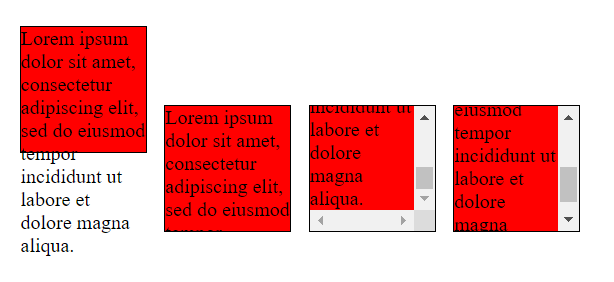
\includegraphics[width=11cm]{ss/overflow.png}
\end{figure}


\subsection{z-index}

Cuando una etiqueta se sobrepone en otra es debido a que, en el DOM y código HTML, la sobrepuesta va después de la que está por debajo, esto siempre ocurre, pero podemos cambiar el orden en el que se posicionan los elementos sobrepuestos. La propiedad \textbf{z-index} de CSS recibe como valores números enteros y da como resultado un ordenamiento de elementos sobrepuestos distinta. Veamos el siguiente código y su resultado (\textit{Figura \ref{fig: 32}}):
\begin{lstlisting}
estilos.css
    /* El primer contenedor tiene el "z-index" de 2. */
    .cont1 {
        position: fixed;
        top: 100px;
        left: 100px;
        width: 150px;
        height: 150px;
        background-color: red;
        /* "z-index" 2. */
        z-index: 2;
    }
    /* El segundo contenedor tiene el "z-index" de 1. */
    .cont2 {
        position: fixed;
        top: 180px;
        left: 180px;
        width: 150px;
        height: 150px;
        background-color: blue;
        color: white;
        /* "z-index" 1 */
        z-index: 1;
    }

prueba.html
    <div class="cont1">
        <p>Contenedor 1</p>
    </div>
    <div class="cont2">
        <p>Contenedor 2</p>
    </div>
\end{lstlisting}
\begin{figure}[H]
    \centering
    \caption{Funcionamiento de la propiedad \textit{z-index}}
    \label{fig: 32}
    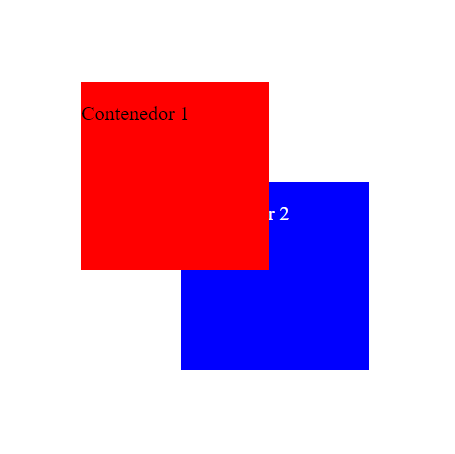
\includegraphics[width=7cm]{ss/z-index.png}
\end{figure}

Como vemos, el primer div con la clase "cont1" aparece, después, el siguiente div con la clase "cont2" aparece, ambos con la propiedad \textit{position} "fixed", el segundo div se sobrepone al primero por defecto, sin embargo, el estilo CSS le da a la clase "cont1" el valor 2 de \textit{z-index} y el valor 1 a la clase "cont2", por lo que "cont1" se sobrepone. No olvidar que la propiedad \textit{z-index} solamente funciona con elementos con la propiedad \textit{position} y el valor \textit{absolute}, \textit{relative} y \textit{fixed}.
